\documentclass{article} % класс документа
%Преамбула документа
\usepackage{packages}

% Параметры страницы
\textheight=24cm
\textwidth=16cm
\oddsidemargin=5mm
\evensidemargin=-5mm
\marginparwidth=36pt
\topmargin=-2cm
\footskip=2.5em
\footnotesep=2ex
\flushbottom
\raggedbottom
\tolerance 3000
% подавить эффект "висячих стpок"
\clubpenalty=10000
\widowpenalty=10000
\renewcommand{\baselinestretch}{1.1}
\renewcommand{\baselinestretch}{1.5} %для печати с большим интервалом
\title{On the loss landscape in grokking: mode connectivity}

\author{ Грозный С.В \\
	Кафедра ММП, факультет ВМК \\
    МГУ им. М.В. Ломоносова\\
	\texttt{groznysv@my.msu.ru} \\
	%% examples of more authors
	\And
    Южаков Т. А.\\
	ФКН, НИУ ВШЭ\\
    Исследовательская группа Байесовских методов\\
    \And
    Ветров Д.П.\\
    кандидат ф.-м. наук\\
    Профессор НИУ ВШЭ\\
    Исследовательская группа Байесовских методов\\
	%% Coauthor \\
	%% Affiliation \\
	%% Address \\
	%% \texttt{email} \\
	%% \And
	%% Coauthor \\
	%% Affiliation \\
	%% Address \\
	%% \texttt{email} \\
	%% \And
	%% Coauthor \\
	%% Affiliation \\
	%% Address \\
	%% \texttt{email} \\
}
\date{}

\renewcommand{\shorttitle}{On the loss landscape in grokking: mode connectivity}

%%% Add PDF metadata to help others organize their library
%%% Once the PDF is generated, you can check the metadata with
%%% $ pdfinfo template.pdf
% \hypersetup{
% pdftitle={A template for the arxiv style},
% pdfsubject={q-bio.NC, q-bio.QM},
% pdfauthor={David S.~Hippocampus, Elias D.~Striatum},
% pdfkeywords={First keyword, Second keyword, More},
% }

\begin{document}
\maketitle
\begin{abstract}
	В данной работе исследован эффект гроккинга в глубоком обучении, представляющий собой интересную тенденцию, при которой нейронные сети достигают 100\% точности на обучающей выборке, сохраняя при этом случайный уровень точности на отложенной выборке, а затем внезапно достигают 100\% точности на ней. Было предложено анализировать ландшафт функции потерь, используя пути, соединяющие оптимумы, для объяснения этого явления. В результате исследования было выявлено, что сложная структура ландшафта функции потерь в гроккинге объясняется блужданием по многообразию функции потерь с нулевой ошибкой, начиная с узкого минимума и переходя к более широкому, что способствует улучшению обобщающей способности модели. Кроме того, было показано, что использование определенных кривых для соединения оптимумов может существенно снизить ошибку на отложенной выборке. Эти результаты могут иметь важное значение для оптимизации и эффективного обучения глубоких нейронных сетей.
\end{abstract}
\section{Введение}
Глубокие нейронные сети стали мощным инструментом для обработки сложных данных и решения разнообразных задач: от классификации изображений до генерации текста. Однако, оптимизация и эффективное обучение таких моделей остаются актуальными проблемами.

Также, в процессе развития глубокого обучения обнаруживают всё больше и больше необычных явлений, которые трудно объяснить. Сложность заключается в том, что модели в последнее время имеют миллионы, а то и миллиарды параметров, и поэтому высокая размерность функции потерь влечет за собой трудности в ее интерпретации. Понимание геометрических свойств поверхности функции потерь может помочь в поиске причин возникновения данных явлений и построении более эффективных процедур обучения. 

В данной работе исследование ландшафта функции потерь будем проводить на примере т.н. эффекта гроккинга\cite{power2022grokking}. Его суть заключается в том, что даже при достижении нулевой ошибки на обучении в сети продолжают происходить процессы упорядочивания информации. Попробуем объяснить это через анализ ландшафта функции потерь с помощью построения путей, связывающих оптимумы. 
\section{Эффект гроккинга}
Гроккинг - это любопытная тенденция обобщения для нейронных сетей, обученных на определенных алгоритмических задачах. При гроккинге график точности (и потерь) сети показывает две фазы (Рис. \ref{fig:grokking_acc}). В начале обучения точность обучения достигает 100\%, в то время как точность на отложенной выборке остается близкой к случайной (т.е. запоминание обучающей выборки). Значительно позже в процессе обучения точность обобщения внезапно подскакивает до 100\%. Отметим, что если обучать модель без коэффициента регуляризации, то эффекта гроккинга не будет. 
\begin{figure}[!ht]
    \centering
    \subfloat{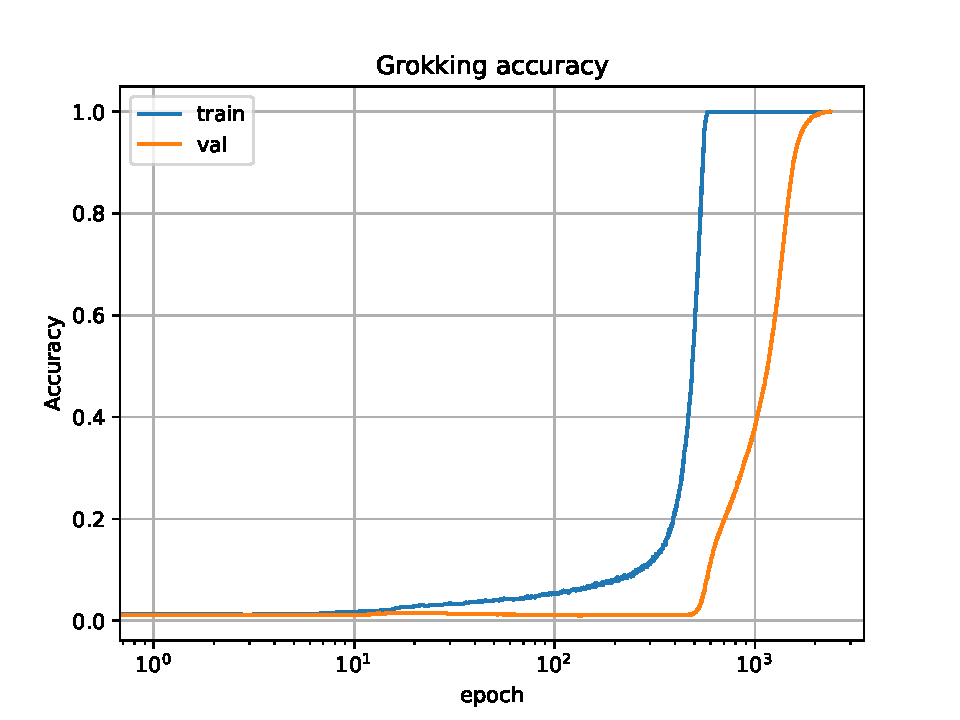
\includegraphics[width = 0.5\textwidth]{figures/grokking_acc.pdf}}
    \subfloat{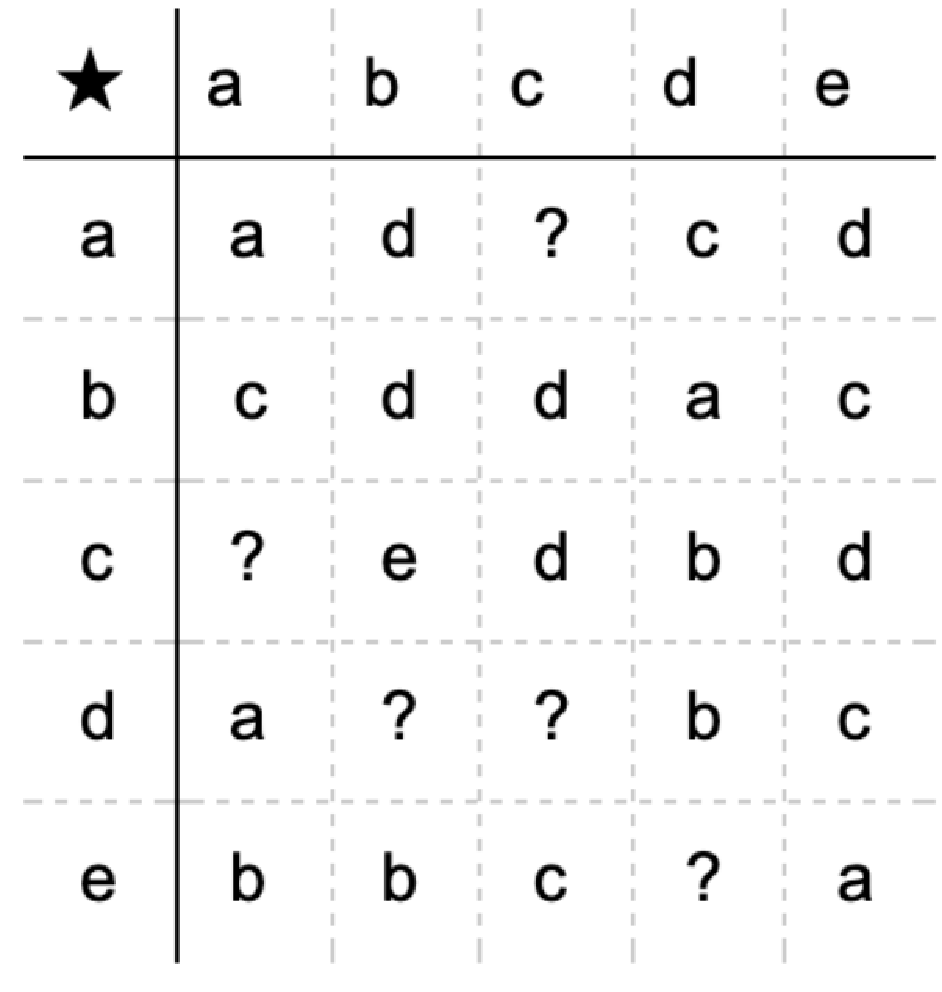
\includegraphics[scale = 0.37]{figures/table.pdf}}
    \caption{\textbf{Слева}: Точность: однослойный decoder-only трансформер, оптимизатор SGD с параметрами lr=0.1, weight decay=0.001. \textbf{Справа}: Сгенерированные данные, поделенные на train и test(знак ?).}
    \label{fig:grokking_acc}
\end{figure}
\subsection{Описание данных}
Этот эффект можно пронаблюдать на данных следующего вида: $a\circ b=c$, где $a, b, c$ - числа, а $\circ$ - некая бинарная операция. Составляется таблица (Рис. \ref{fig:grokking_acc}), где строки и столбцы это всевозможные значения $a$ и $b$, в ячейках которой хранятся соответствующие этим $a$ и $b$ - $c$. Далее, случайным образом стираются некоторые ячейки(то есть разбиваем выборку на train и test(пустые ячейки)). Задача состоит в том, чтобы заполнить пустые ячейки в соответствии с выше описанной операцией.

Для экспериментов в качестве бинарной операции возьмем умножение по модулю 97 : $x * y \pmod{97}$. Пусть $x \in [ \, 0, 96 ] \,$, $y \in [ \, 1, 96 ]$, а результат операции, очевидно, лежит на $[ \, 0, 96 ] \,$. 
\subsection{Описание модели и метода оптимизации}
Авторы оригинальной статьи разбивают $a\circ b=c$ на 5 токенов: $a, \circ, b, =, c$. Для экспериментов будет достаточно только три токена: $a, b, c$, так как это обеспечивает более стабильное обучение. 

Сопоставим каждому числу от 0 до 96 соответствующий вектор эмбеддинга размерности 128, а после применяем однослойный decoder-only трансформер без нормализации из статьи \textit{omnigrok}\cite{liu2023omnigrok}. В качестве стратегии оптимизации будем использовать стохастический градиентый спуск с темпом обучения 0.01, коэффициентом регуляризации 0.001 и размером батча 512.
\section{Связность оптимумов нейронных сетей}
Как известно \cite{garipov2018loss}, глобальные оптимумы, в которых достигается нулевая ошибка на обучении, образуют многообразие нулевого трейн лосса. Попробуем построить путь, соединяющий эти оптимумы и исследуем поведение функции потерь по мере его прохождения. Для начала введем несколько определений. 
\\~\\
\textbf{Опр. 1} \textit{Пусть $w_1$, $w_2 \in \mathbb{R}^n$. Отображение вида} 
$$\phi(t): [ \, 0, 1 \, ] \rightarrow \mathbb{R}^n $$
\textit{такое, что $\phi(0)=w_1, \phi(1)=w_2$, будем называть \textbf{путем}, соединяющим точки $w_1$ и $w_2$.}
\\~\\
Самый простой путь, который можно построить - это отрезок. Определим его в контексте нашей задачи.
\\~\\
\textbf{Опр. 2} \textit{Пусть $w_1$, $w_2 \in \mathbb{R}^n$. Функцию вида} 
$$\phi(t) = tw_1+(1-t)w_2, \, t \in [0, 1]$$
\textit{будем называть \textbf{отрезком}, соединяющим точки $w_1$ и $w_2$.}
\\~\\
Также, попробуем соединить оптимумы такой кривой, чтобы значение функции потерь было минимально. \\
Метод поиска этой кривой между парой оптимумов интуитивно очень прост: параметризуем путь и минимизируем средние потери на этом пути относительно его параметров. Точнее, минимизируем
$$L(\theta)= \int_{0}^{1} Loss(\phi_{\theta}(t)) \,dt = E_{t \sim U [ 0, 1 ]} Loss(t)$$
по $\theta$, где $Loss$ - функция потерь. \\
Также есть способ эффективно вычислять стохастические градиенты $L(\theta)$ по $\theta$. Для этого выбираем точку $t$ из равномерного распределения на отрезке $[0,1]$, а зачем вычисляем градиент $Loss(\theta)$ по $\theta$, используя правило цепочки:
$$\frac{\partial Loss(\phi(t))}{\partial \theta} = \frac{\partial Loss(\phi(t))}{\partial \phi(t)}\frac{\partial \phi(t)}{\partial t}$$
Используя эту стохастическую оценку градиента, происходит минимизация $L(\theta)$ с помощью стандартного SGD. \\
В экспериментах в качестве параметризованной кривой будем использовать ломаную с одним изгибом. 
\\~\\
\textbf{Опр. 3} \textit{Пусть $w_1$, $w_2$, $\theta  \in \mathbb{R}^n$. Функцию вида} 
%$$\phi(t) = 2 (t\theta + (0.5 − t)w_1), 0 \le t \le 0.5$$
$$ \phi_{\theta}(t) =
\begin{cases}
\, 2 \, (t\theta + (0.5 - t)w_1) , \quad \quad \, \, \, \, t \in  [ 0,0.5 ] \\
\, 2 \, ((t-0.5)w_2+(1-t)\theta) , \, t \in  [0.5,1 ] \\
\end{cases}
$$
\textit{будем называть \textbf{ломаной с одним изгибом}.}

Исследования показывают \cite{keskar2017largebatch}, что кривизна поверхности функции потерь значительно скоррелирована с обобщающей способностью. Поэтому будем также считать норму стохастичского градиента.
\section{Эксперименты}
Пусть $w_1$ и $w_2$ - веса модели, при которых модель впервые достигла 100\% на обучающей и валидационной выборке соответственно. Если смотреть на график \ref{fig:grokking_acc}, то это соответствует моменту запоминания (будем называть  это точкой 1) и моменту гроккинга (будем называть это точкой 2).

Попробуем соединить эти точки различными способами и посмотрим на поведение графиков функции потерь и ошибки (один минус точность). Также будем считать среднюю норму стохастического градиента, т.е. вычислять все минибатч градиенты по выборке, считаем их норму и после вычисляем среднее данной статистики.
\newpage
\subsection{Исследование линейной связности оптимумов}
Посмотрим, как ведут себя вышеперечисленные метрики, если соединить точку 1 и 2 с помощью отрезка:
\begin{figure}[!ht]
    \centering
    \subfloat{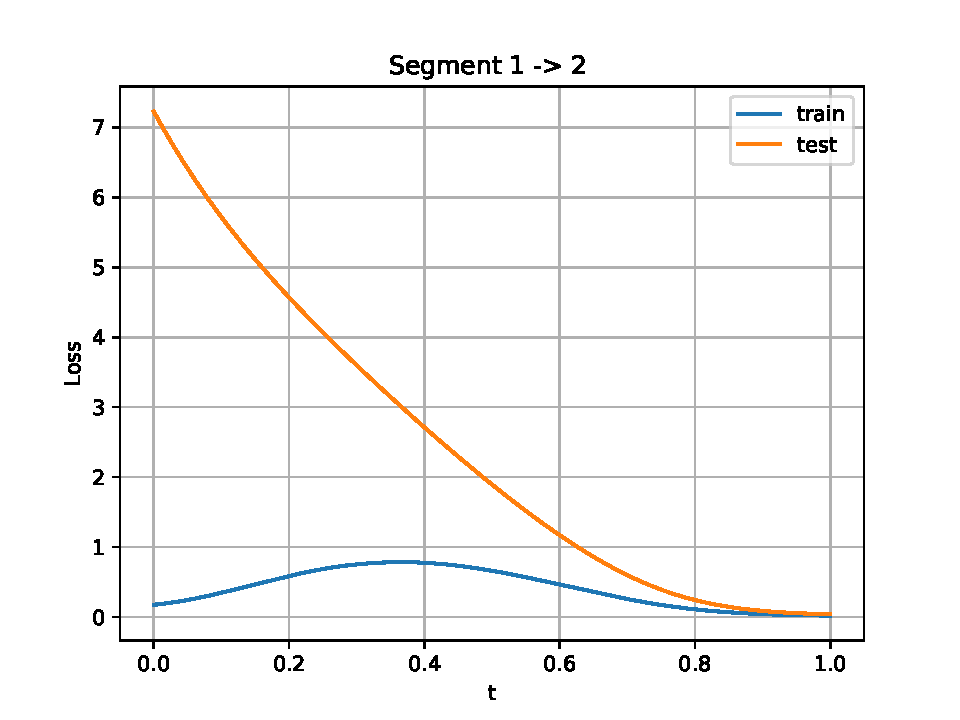
\includegraphics[width = 0.33\textwidth]{figures/1_segment/train_val_loss.pdf}}
    \subfloat{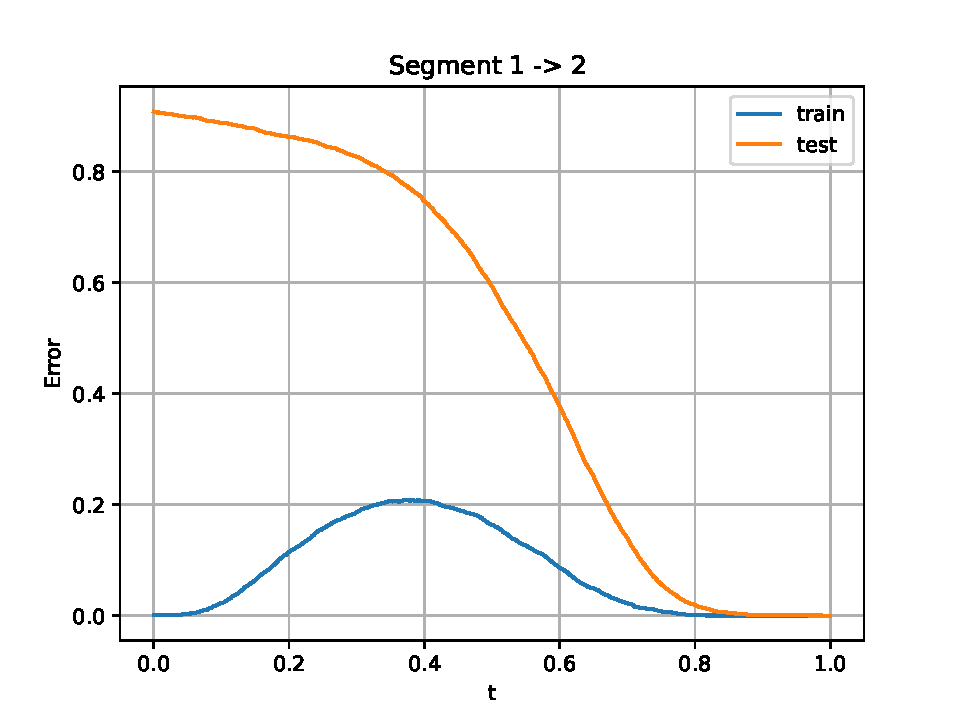
\includegraphics[width = 0.33\textwidth]{figures/1_segment/train_val_err.pdf}}
    \subfloat{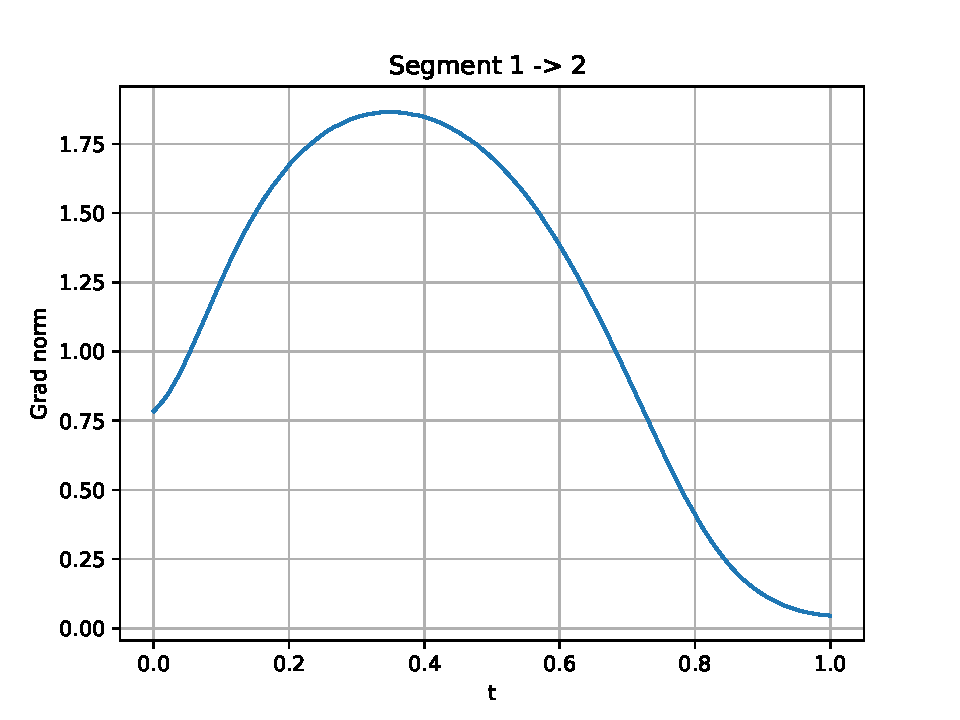
\includegraphics[width = 0.33\textwidth]{figures/1_segment/grad_norm.pdf}}
    \caption{Кросс-энтропия с $l_2$ регуляризацией (\textbf{слева}), ошибка (\textbf{центр}) и норма стох. града (\textbf{справа}) как функции от точек на кривой $\phi(t)$ - отрезок.}
    \label{fig:segment}
\end{figure}

Как и ожидалось, модель показывает просадку точности на обучающей выборке(пик при $t=0.35$). Отметим, что несмотря на это, график на отложенной выборке монотонно падает. Норма градиента перетекает из 0.75 к значению близкому к нулю. 

Можно предположить, что происходит следующее: модель выскакивает из узкого минимума и, двигаясь по сложному рельефу функции потерь, попадает в широкий минимум.
\subsection{Исследование нелинейной связности оптимумов}
\subsubsection{Соединение последовательными отрезками}
\begin{figure}[!ht]
    \centering
    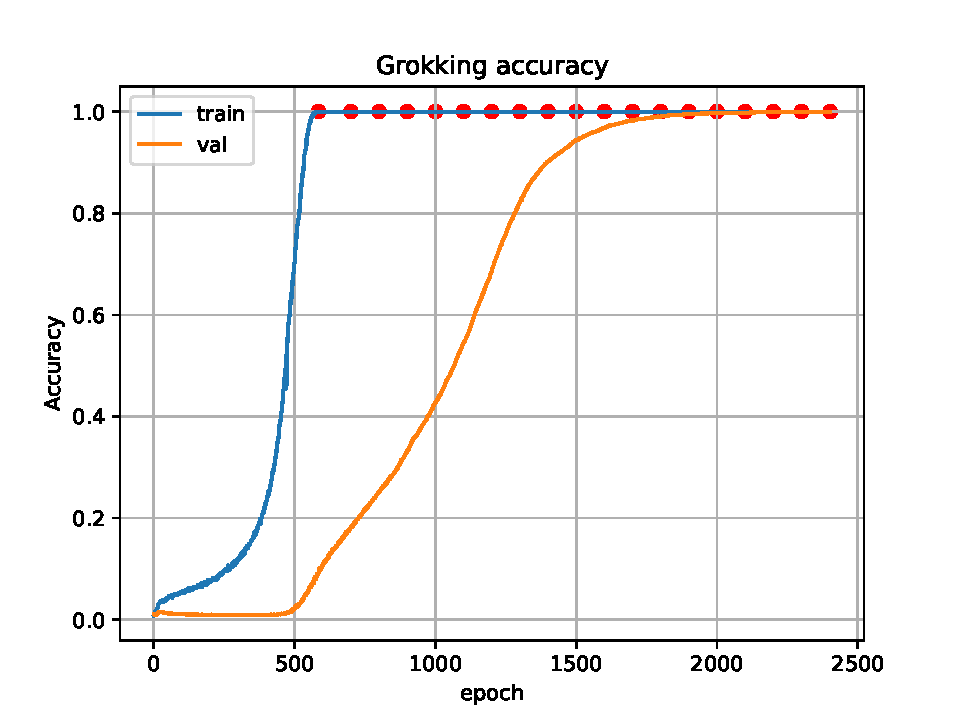
\includegraphics[scale=0.5]{figures/many_segments/grokking_acc.pdf}
    \caption{Однослойный decoder-only трансформер, оптимизатор SGD с параметрами lr=0.1, weight decay=0.001, логирование весов модели каждые сто эпох (красные круги).}
    \label{fig:grokking_acc_many}
\end{figure} 
В данном эксперименте построим путь от точки 1 до точки 2 с помощью последовательно соединенных отрезков. Для этого фиксируем веса каждые 100 эпох и последовательно соединяем. Продемонстрируем графики только для первого и последнего отрезка:
\begin{figure}[!ht]
    \centering
    \subfloat{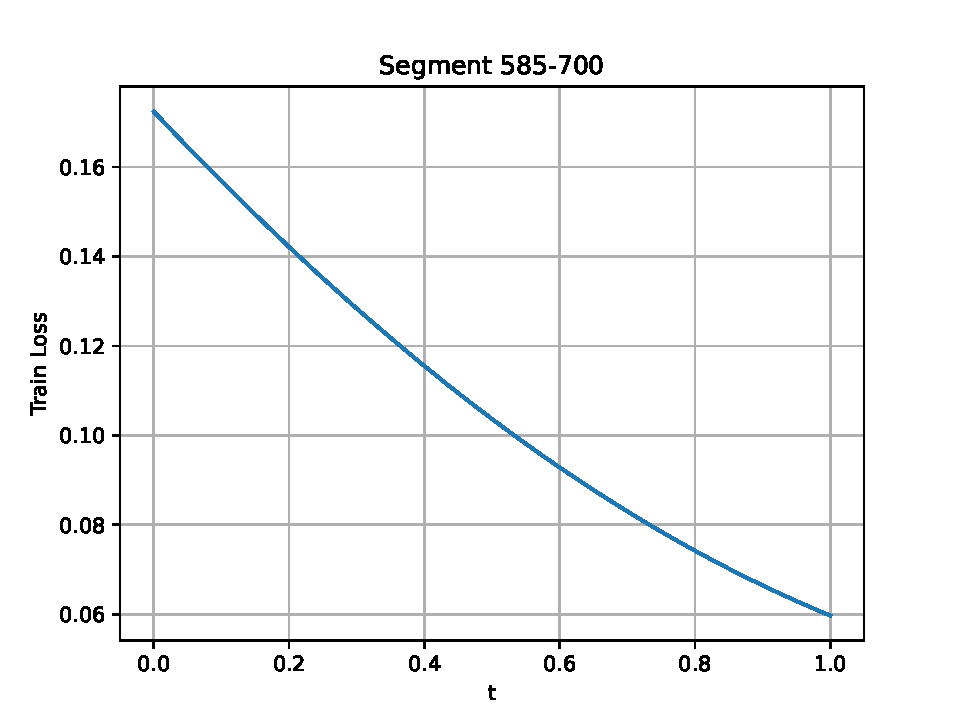
\includegraphics[width = 0.3\textwidth]{figures/many_segments/first/train_loss_585_700.pdf}}
    \subfloat{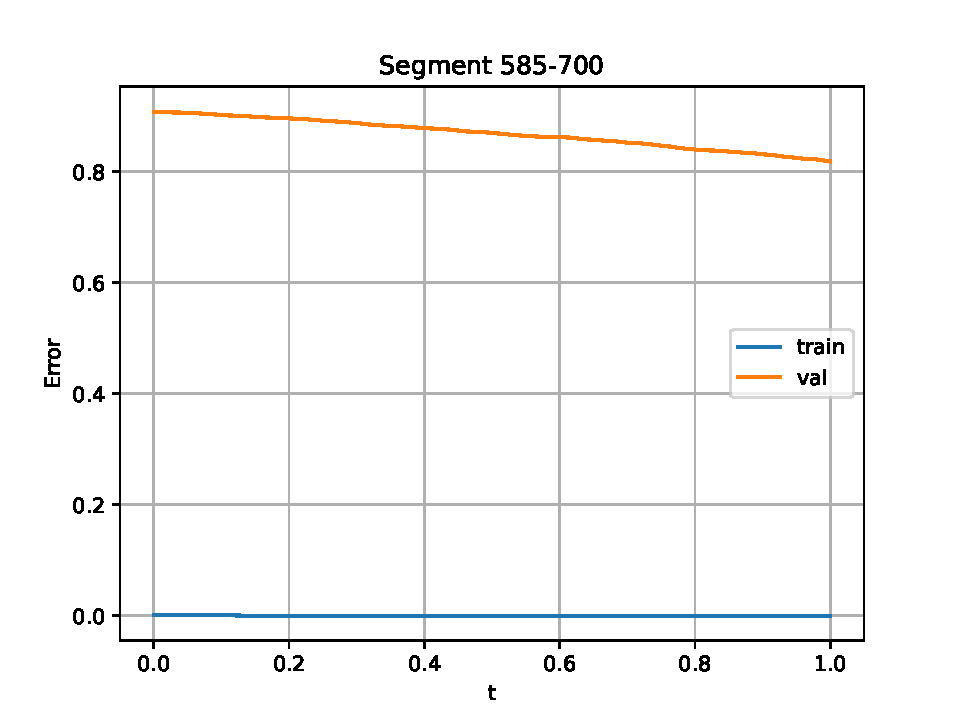
\includegraphics[width = 0.3\textwidth]{figures/many_segments/first/train_val_err_585_700.pdf}}
    \subfloat{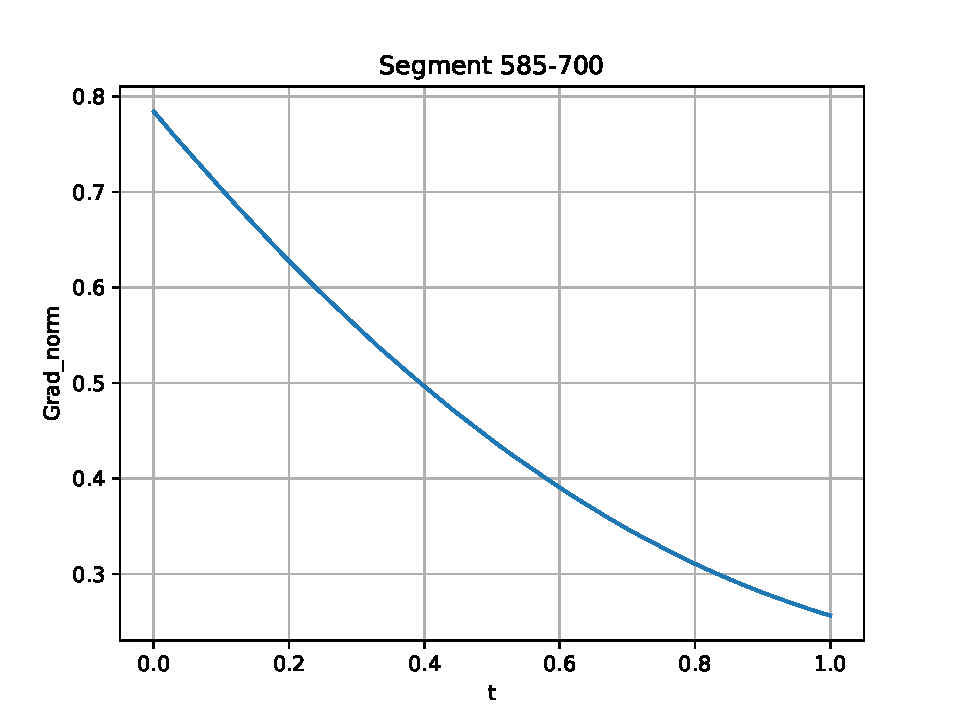
\includegraphics[width = 0.3\textwidth]{figures/many_segments/first/grad_norm_585_700.pdf}} \\
    \centering
    \subfloat{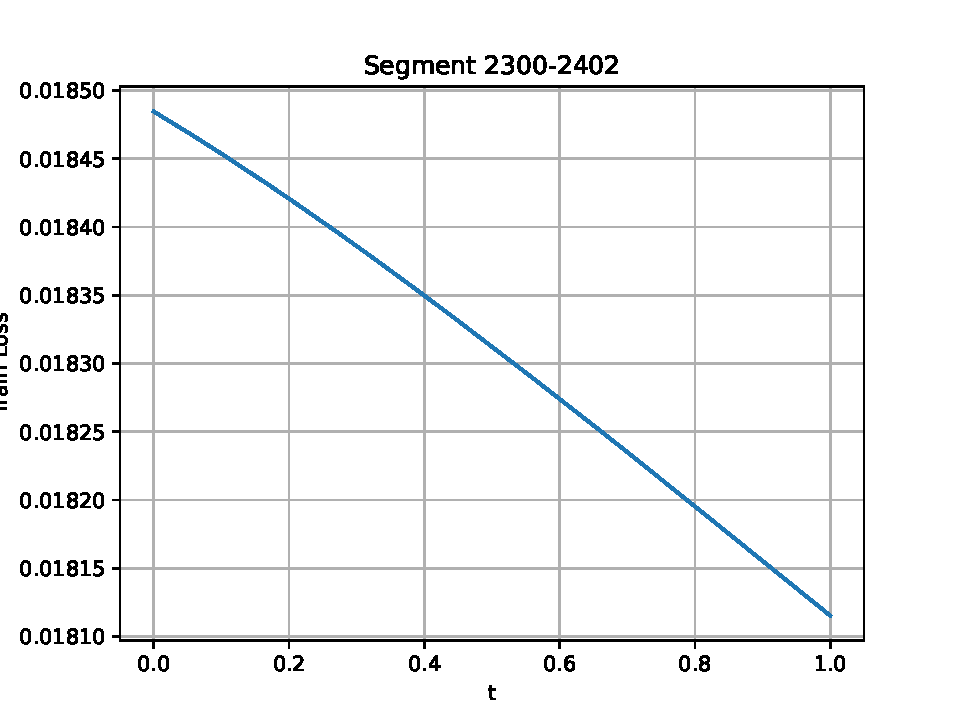
\includegraphics[width = 0.3\textwidth]{figures/many_segments/second/train_loss_2300_2402.pdf}}
    \subfloat{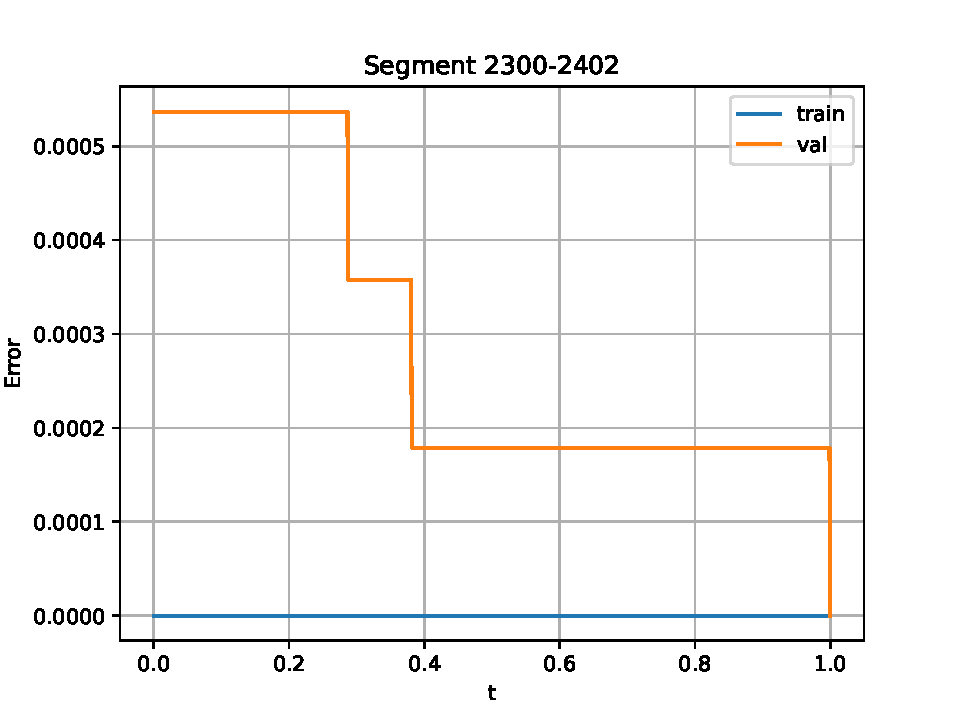
\includegraphics[width = 0.3\textwidth]{figures/many_segments/second/train_val_err_2300_2402.pdf}}
    \subfloat{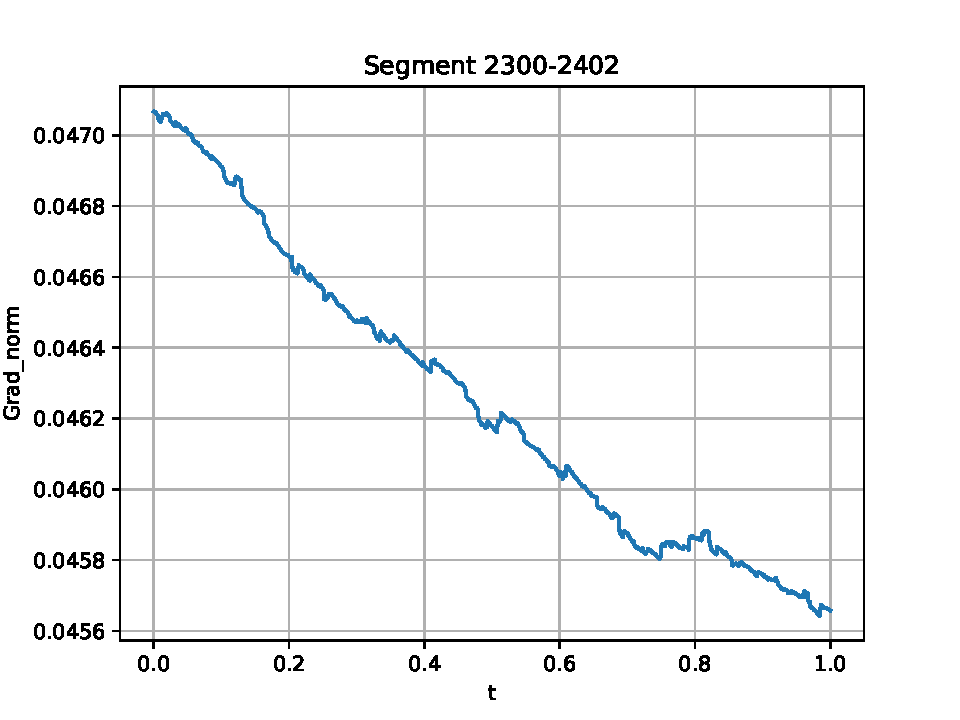
\includegraphics[width = 0.3\textwidth]{figures/many_segments/second/grad_norm_2300_2402.pdf}}
    \caption{\textbf{1 ряд}: отрезок, соединяющий 585 и 700 эпоху. \textbf{2 ряд}: отрезок, соединяющий 2300 и 2402 эпоху. 585 и 2402 эпохи соответствуют 100\% точности на обучающей, низкой на отложенной и 100\% на отложенной,  100\% на  обучающей выборке соответственно.}
    \label{fig:many_segments}
\end{figure}

Как можно заметить, на первом отрезке происходит существенное изменение функции потерь и нормы градиента, а на последнем изменения незначительные. Удивительно, что на протяжении всего пути ошибка на обучающей выборке нулевая. 

Таким образом, удалось соединить два оптимума последовательными отрезками с констатно нулевой ошибкой. Из этого можно сделать вывод, что после запоминания обучающей выборки происходит дрейфование по многообразию нулевого трейн лосса.
\subsubsection{Соединение ломаной с одним изгибом}
Теперь попробуем соединить оптимумы с помощью одной параметризованной кривой, а именно ломаной с одним изгибом. Причем, соединять оптимумы будем не только соответствующие точкам 1 и 2, но и полученных при различных начальных инициализациях. Далее за точки 1 и 1' будем обозначать момент первого достижения 100\% точности на обучающей выборке при разных инициализациях соответственно. Аналогично определяются точки 2 и 2', как точки первого достижения 100\% на валидации.

Ранее удалось соединить точки 1 и 2 несколькими отрезками с нулевой ошибкой. Посмотрим, как ведут себя метрики на кривой, подобранной с помощью оптимизиации.
\begin{figure}[!ht]
    \centering
    \subfloat{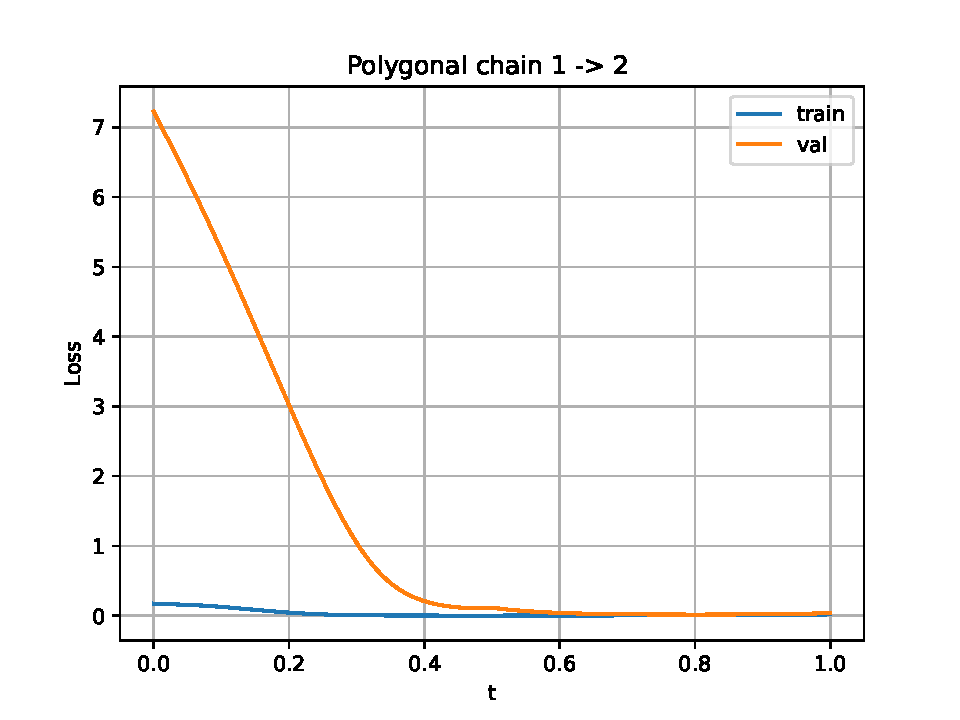
\includegraphics[width = 0.33\textwidth]{figures/pol_chain12/train_val_loss.pdf}}
    \subfloat{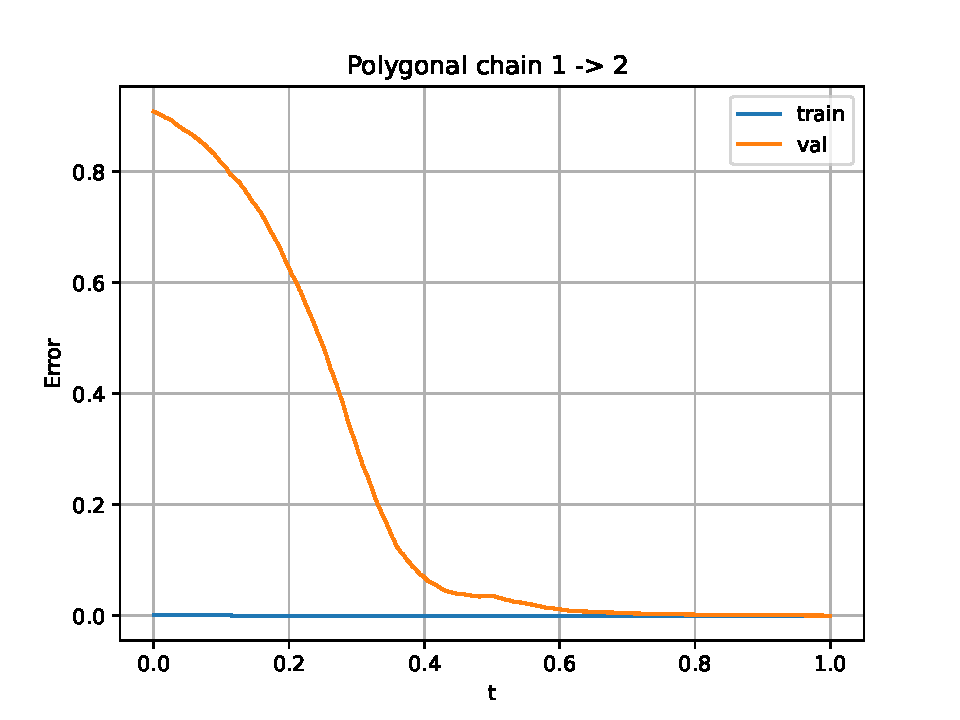
\includegraphics[width = 0.33\textwidth]{figures/pol_chain12/train_val_err.pdf}}
    \subfloat{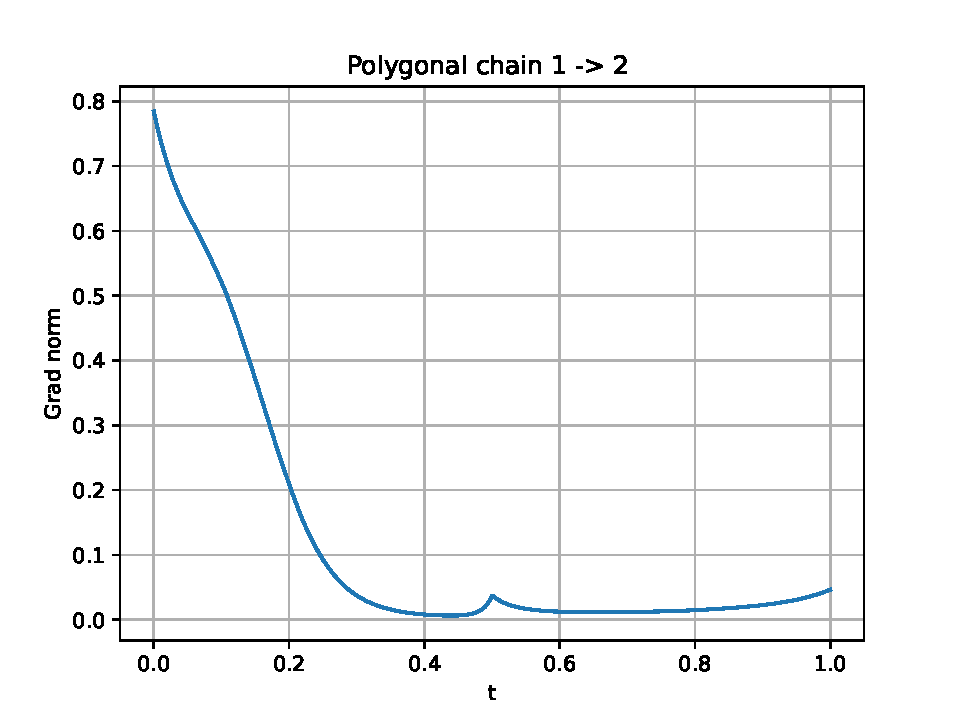
\includegraphics[width = 0.33\textwidth]{figures/pol_chain12/grad_norm.pdf}}
    \caption{Кросс-энтропия с $l_2$ регуляризацией (\textbf{слева}), ошибка (\textbf{центр}) и норма стох. града (\textbf{справа}) как функции от точек на кривой $\phi_{\theta}(t)$ - ломаная с одним изгибом.}
    \label{fig:pol_chain12}
\end{figure}
По графику (Рис. \ref{fig:pol_chain12}) ошибки на обучающей выборке можно убедиться, что оптимизация параметра $\theta$ произошла успешна. Также по графику нормы градиента видно, как из узкого минимума переходим в широкий. 

Заметим, что по сравнению с отрезком (Рис. \ref{fig:segment}), выйти на плато хорошего качества на валидации удалось значительно раньше: с момента $t=0.6$.

Теперь попробуем построить путь через оптимумы <<запоминания>> обучающей выборки, полученные через разные инициализации. Оптимизируем кривую по параметру $\theta$ и считаем метрики:
\begin{figure}[!ht]
    \centering
    \subfloat{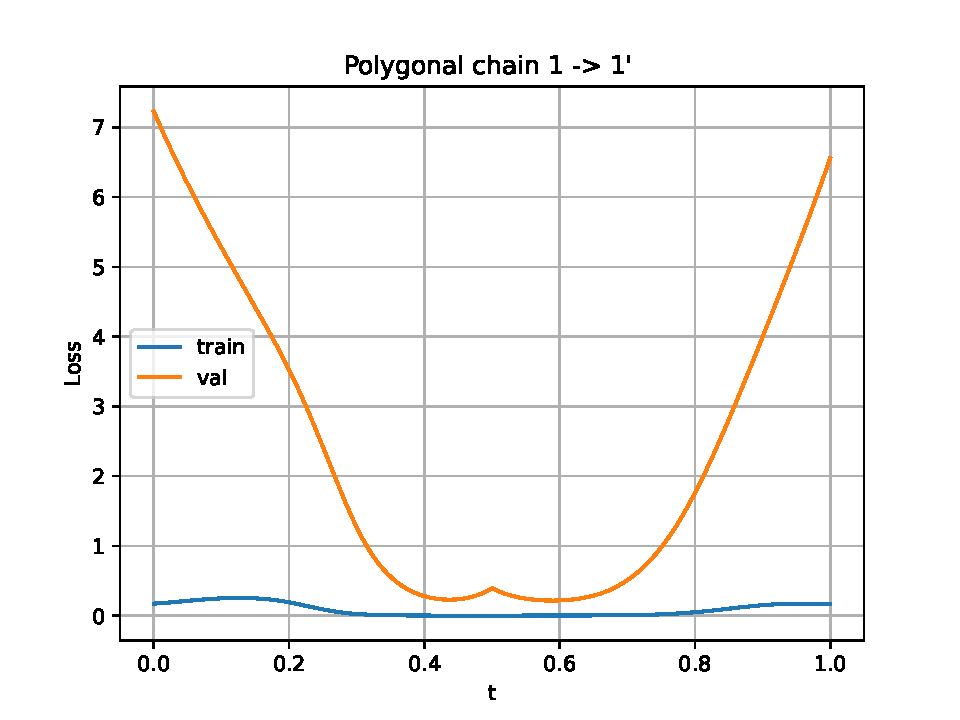
\includegraphics[width = 0.33\textwidth]{figures/pol_chain11/train_val_loss.pdf}}
    \subfloat{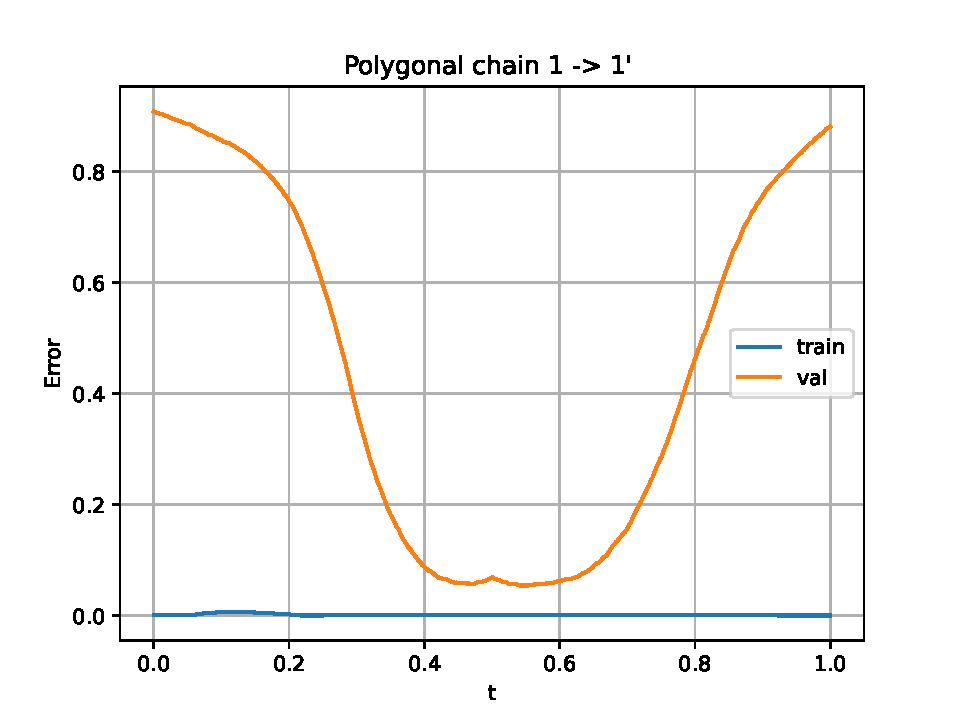
\includegraphics[width = 0.33\textwidth]{figures/pol_chain11/train_val_err.pdf}}
    \subfloat{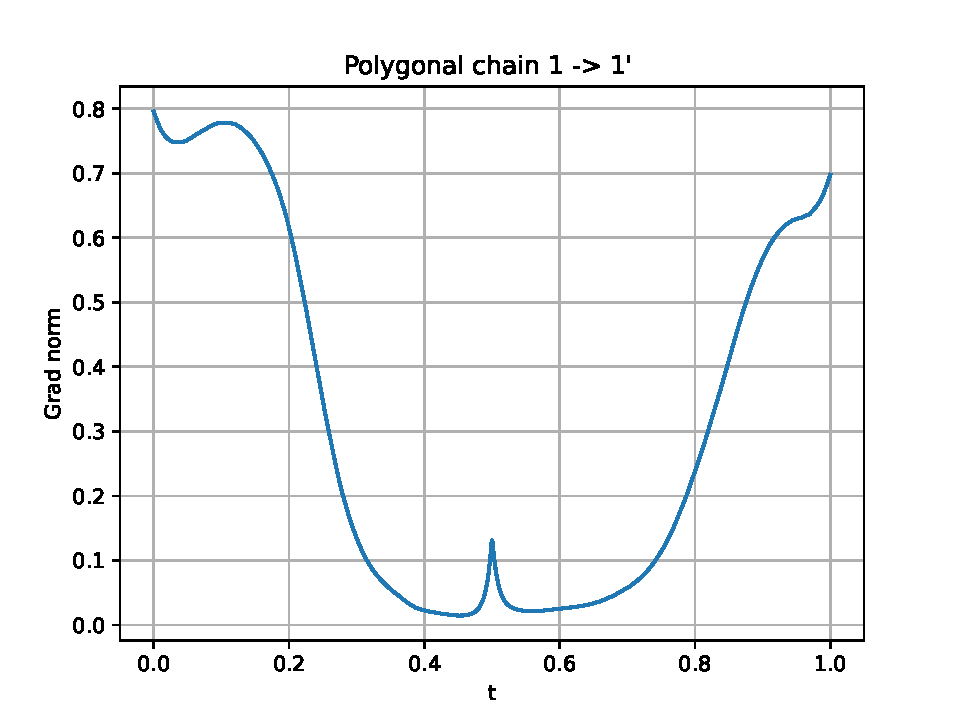
\includegraphics[width = 0.33\textwidth]{figures/pol_chain11/grad_norm.pdf}}
    \caption{Кросс-энтропия с $l_2$ регуляризацией (\textbf{слева}), ошибка (\textbf{центр}) и норма стох. града (\textbf{справа}) как функции от точек на кривой $\phi(t)$. 1 и 1' - точки 100\% точности на обуч. выборке при разных инициализациях.}
    \label{fig:pol_chain11}
\end{figure}

Точность на обучающей выборке показывает, что оптимизация кривой по параметру удалась. Также, наблюдается довольно необычный эффект: при соединении оптимумов с высокой валидационной ошибкой по пути встречается довольно широкий минимум с хорошим обобщением (это особенно заметно в окрестности точки $t=0.5$). 
\newpage

Проведем аналогичный эксперимент, но для точек, соответствующих 100\% точности на валидации:
\begin{figure}[!ht]
    \centering
    \subfloat{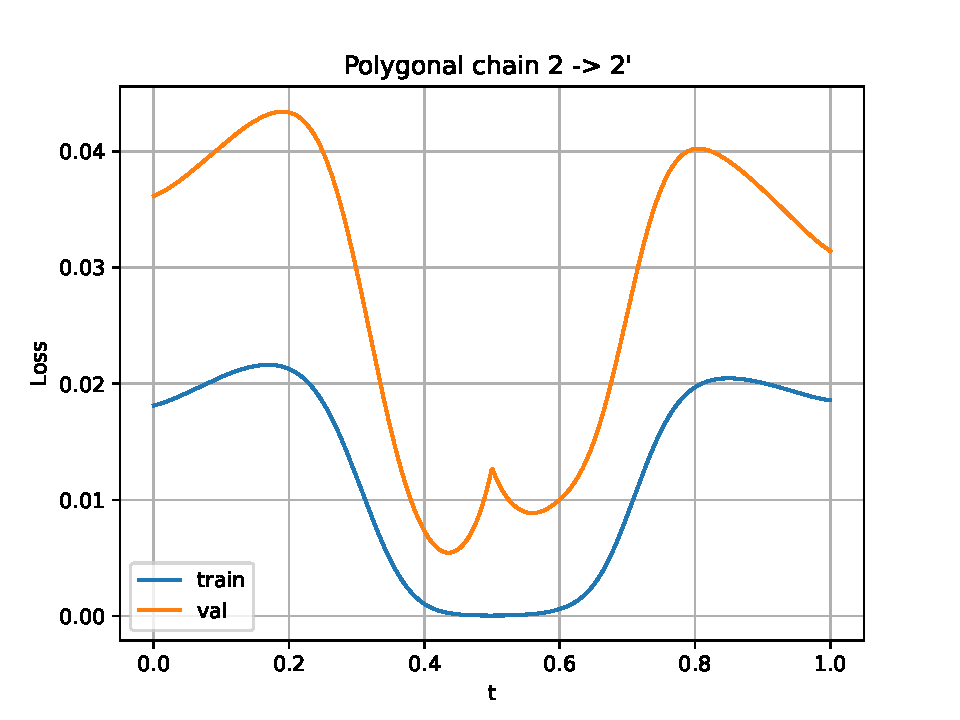
\includegraphics[width = 0.33\textwidth]{figures/pol_chain22/train_val_loss.pdf}}
    \subfloat{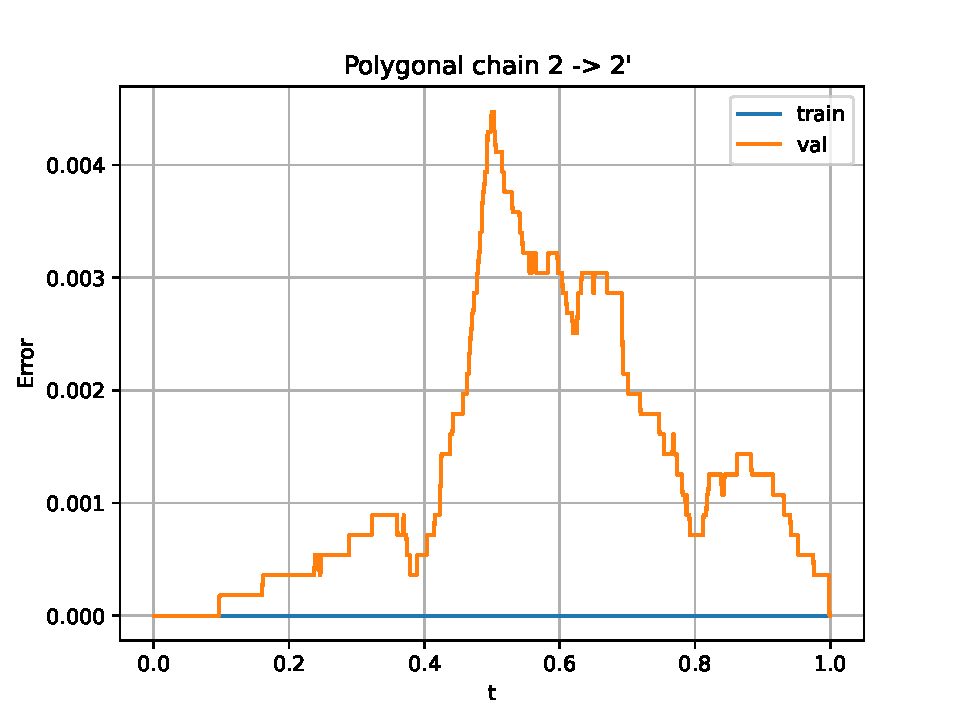
\includegraphics[width = 0.33\textwidth]{figures/pol_chain22/train_val_err.pdf}}
    \subfloat{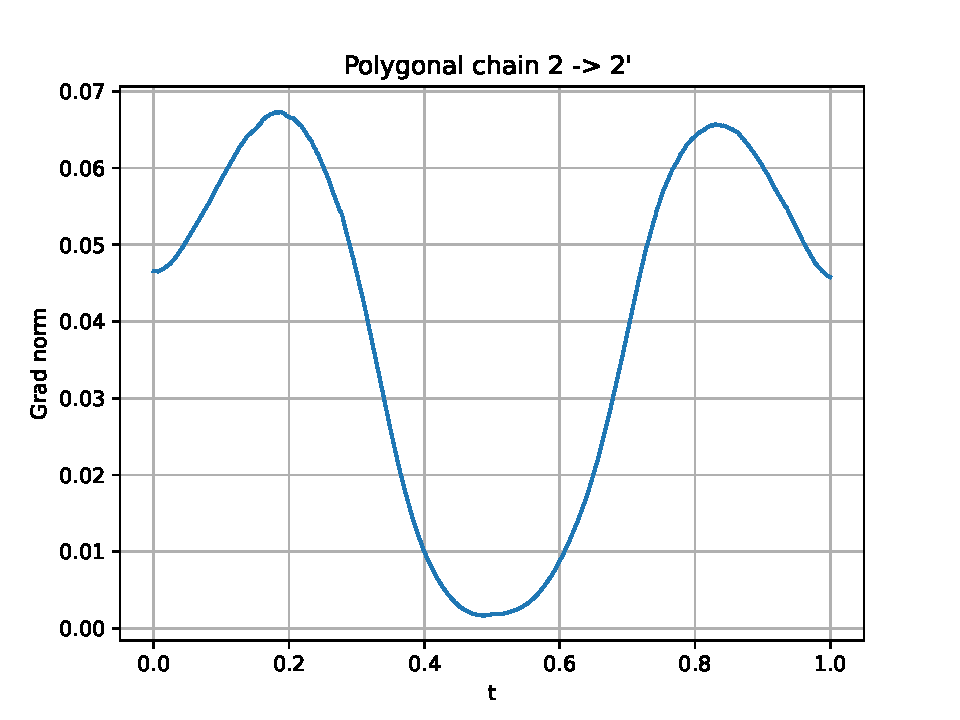
\includegraphics[width = 0.33\textwidth]{figures/pol_chain22/grad_norm.pdf}}
    \caption{Кросс-энтропия с $l_2$ регуляризацией (\textbf{слева}), ошибка (\textbf{центр}) и норма стох. града (\textbf{справа}) как функции от точек на кривой $\phi(t)$. 2 и 2' - точки 100\% точности на вал. выборке при разных инициализациях.}
    \label{fig:pol_chain22}
\end{figure}

Первое, что бросается в глаза, это довольно маленькое изменение значений метрик на кривой. Из этого можно сделать вывод, что два оптимума с хорошим обобщением в задаче гроккинга соединимы с низкой ошибкой на валидации. Также отметим, что график нормы градиента содержит в себе два симметричных холма. Можно сделать предположение, что, двигаясь по кривой, модель сначала выскакивает из минимума, а после в него же и возвращается. 
\section{Выводы}
В данной работе было показано, что ландщафт функции потерь в задаче гроккинга имеет сложную структуру: при соединении двух оптимумов одним отрезком функция потерь показывает просадку в точности. Однако если использовать более сложные кривые, то построение пути с низкой ошибкой на обучающей выборке не составляет труда.

Также, по построению нескольких отрезков, соединяющих оптимумы, можно сделать вывод, что гроккинг возникает в силу блуждания по многообразию функции потерь с нулевой ошибкой. Сначала модель скатывается в узкий минимум, а после переходит в более широкий, где лучше обобщающая способность.

Кроме того, с помощью построения ломаной с одним изгибом удалось достичь довольно низкую ошибку на отложенной выборке, стартуя из точки с низкой валидацией. Если данный эффект удасться повторить на других задачах, то данную оптимизацию можно использовать как менее вычислительно затратную. 
\newpage
\bibliographystyle{plain}
\bibliography{sample.bib}
%\printbibliography[title={Reference}]

%\section{Список используемой литературы}

\end{document}